\chapter{Caracter\'isticas de la Interfaz}
   \label{Caracteristicas_Interfaz}

\section{Primera Ejecuci\'on}
   \label{Primera_Ejecucion}

La primera vez que ejecute \textsc{XLogo} (o si ha borrado el fichero
\texttt{.xlogo} -- ver secci\'on \ref{Desinstalar}) deber\'a elegir
el idioma con que quiere trabajar, seleccionando la bandera correspondiente
y haciendo \textit{click} en el bot\'on \texttt{OK}.
\begin{center}
   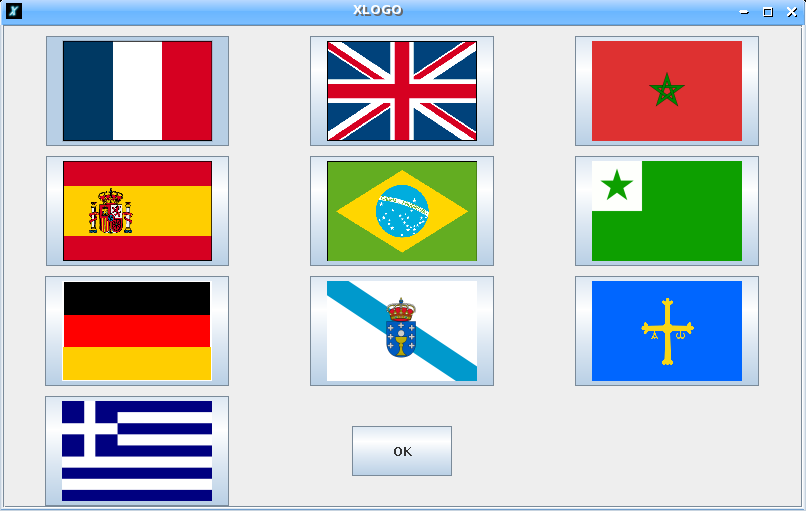
\includegraphics[scale=0.2]{Imagenes/02_Caracteristicas/PantallaIdioma.png}
\end{center}
Esta elecci\'on no es definitiva; puede elegir otro idioma en cualquier
momento desde las opciones de men\'u (secci\'on \ref{Menu-Herramientas})

\section{La ventana principal}
   \label{La-ventana-principal}

\begin{center}
   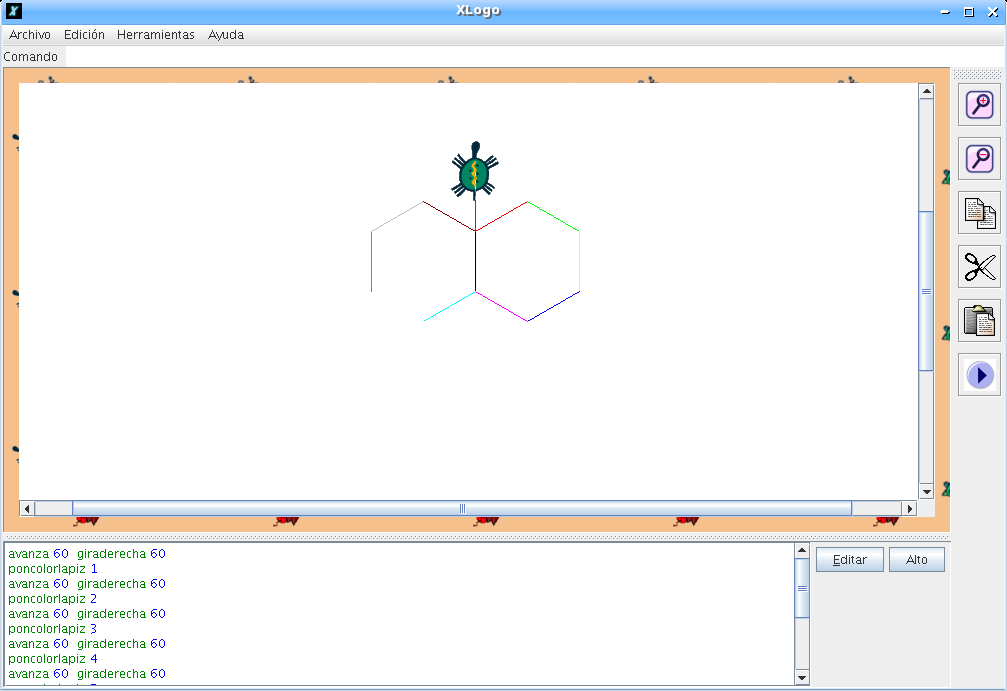
\includegraphics[scale=0.35]{Imagenes/02_Caracteristicas/VentanaPcpal_090.png}
\end{center}

\begin{itemize}
   \item En la fila superior, est\'an las entradas t\'ipicas de men\'u:
      \textbf{Archivo}, \textbf{Edici\'on}, \textbf{Herramientas},
      \textbf{Ayuda}
   \item Justo debajo est\'a la 
      \textbf{L\'inea de Comando},\index{L\'inea de Comando}
      donde se escriben las instrucciones \textsc{Logo}.
   \item En el medio de la pantalla, est\'a el
      \textbf{\'Area de Dibujo} \index{Area@\'Area de Dibujo}
      (donde se mueve la tortuga).
   \item A la derecha del \'area de dibujo se encuentra una barra de
      herramientas vertical con las funciones \textit{zoom}\index{Zoom}
      (acercar y alejar), \textit{copiar},\index{Copiar}
      \textit{cortar}\index{Cortar}, \textit{pegar}\index{Pegar} y
      \textit{Comando de Inicio}\index{Comando de Inicio}.
   \item Al pie, est\'a la ventana del
      \textbf{Hist\'orico de Comandos},\index{Hist\'orico de Comandos}
      que muestra todo lo ingresado y sus respuestas asociadas. Para
      reutilizar un comando previamente ingresado, hay dos opciones:
      Hacer un \textit{click} en un comando del hist\'orico, o usar
      las teclas de flecha arriba y flecha abajo del teclado (lo que
      es m\'as pr\'actico).
   \item A la derecha de la ventana del hist\'orico hay dos botones:
      \textbf{Editar} y \textbf{Alto}. 
      \begin{itemize}
         \item \textbf{Editar} \index{Editar} permite abrir la ventana del
            editor de procedimientos. 
         \item \textbf{Alto} \index{Alto} interrumpe la ejecuci\'on del
            programa ingresado.
      \end{itemize}
\end{itemize}

\section{El editor de procedimientos}
   \label{EditorProcedimientos}
   \index{Editor de Procedimientos}

\begin{center}
   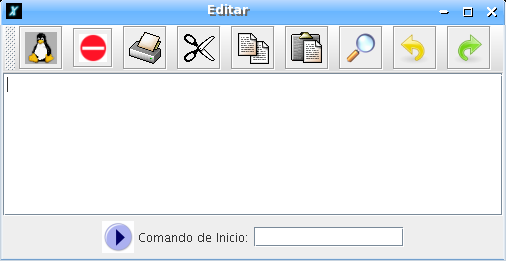
\includegraphics[scale=0.5]
      {Imagenes/02_Caracteristicas/EditorProc_092.png}
\end{center}

Hay cuatro maneras de abrir el editor:
\begin{itemize}
   \item Escribir \texttt{editatodo}\index{editatodo@\texttt{editatodo}} o
      \texttt{edtodo}\index{edtodo@\texttt{edtodo}} en la
      \textbf{L\'inea de Comando}. La ventana del editor se abrir\'a
      mostrando todos los procedimientos definidos hasta ese momento.
   \item Si deseas editar un procedimiento en especial (o algunos), debes
      usar \texttt{ed}\index{ed@\texttt{ed}} o \texttt{edita}\index{edita@\texttt{edita}}
      en la l\'inea de comandos seguido del nombre de procedimiento, o la lista con los
      nombres de procedimientos que deseas editar: \\
      \texttt{edita \char`\"{}nombre\_procedimiento} \\
      o: \\
      \texttt{edita [proc\_1 proc\_2]}
   \item Hacer \textit{click} en el bot\'on \textbf{Editar}.
      \index{Editar}
   \item Usar el atajo de teclado \texttt{Alt+E}
\end{itemize}
Estos son los diferentes botones que encontrar\'as en la ventana del
Editor:
\begin{center} \begin{longtable}{|m{1.3cm}|m{115mm}|} \hline 
   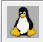
\includegraphics[scale=1.0]{Imagenes/02_Caracteristicas/guardar.png} &
      Guarda en memoria los cambios hechos en el editor y cierra la ventana.
      Es este bot\'on el que se debe usar cada vez que quieras aplicar los
      procedimientos recientemente incorporados.

      Atajo de teclado: \texttt{ALT+Q}. \\ \hline 
   
\includegraphics[scale=1.0]{Imagenes/02_Caracteristicas/salir.png} &
      Cierra la ventana del editor sin guardar los \'ultimos cambios. Ten
      presente que NO aparece ning\'un mensaje de confirmaci\'on. Aseg\'urate
      bien de que realmente no hay nada que guardar.

      Atajo de teclado: \texttt{ALT+C}. \\ \hline 
   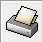
\includegraphics[scale=1.0]{Imagenes/02_Caracteristicas/imprimir.png} & 
      Imprime el contenido del editor.\\ \hline 
   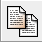
\includegraphics[scale=1.0]{Imagenes/02_Caracteristicas/copiar.png} &
      Copia el texto seleccionado al portapapeles.

      Atajo de teclado: \texttt{Control+C}.\\ \hline 
   
\includegraphics[scale=1.0]{Imagenes/02_Caracteristicas/cortar.png} &
      Corta el texto seleccionado y lo copia al portapapeles.

      Atajo de teclado: \texttt{Control+X}.\\ \hline 
   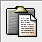
\includegraphics[scale=1.0]{Imagenes/02_Caracteristicas/pegar.png}&
      Pega el contenido del portapapeles.

      Atajo de teclado: \texttt{Control+V}.\\ \hline
   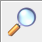
\includegraphics[scale=1.0]{Imagenes/02_Caracteristicas/lupa.png}&
      Permite realizar b\'usquedas y reemplazos en los procedimientos. Para
      ello se abre la ventana siguiente:
      \begin{center}
         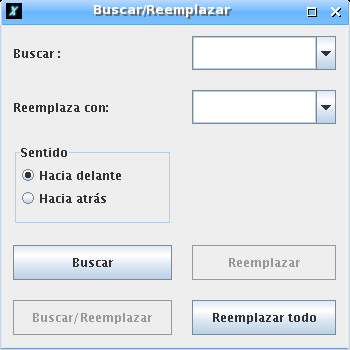
\includegraphics[scale=0.45]{Imagenes/02_Caracteristicas/BuscarReemplazar.png}
      \end{center} \\ \hline
   
\includegraphics[scale=1.0]{Imagenes/02_Caracteristicas/undo.png}&
      Permite deshacer los \'ultimos cambios realizados en los procedimientos.\\ \hline
   
\includegraphics[scale=1.0]{Imagenes/02_Caracteristicas/redo.png}&
      ``Rehace'' lo deshecho con el bot\'on anterior.\\ \hline
\end{longtable} \end{center}

\textbf{Nota:} Aunque aqu\'i se representa la imagen de Tux (mascota de Linux) en el
bot\'on ``\textit{Guardar}'', en realidad se muestra la tortuga activa para dar la
idea de ``\textit{enviar la informaci\'on a la tortuga}''; por ejemplo, si la tortuga
activa es la n\'umero 3 (secci\'on \ref{Menu_Preferencias}):
\begin{center}
   \includegraphics[scale=0.5]{Imagenes/02_Caracteristicas/EditorProc_093.png}
\end{center}

En la parte inferior se encuentra l\'inea donde definir el
\texttt{Comando de Inicio}, que se activa con el bot\'on situado a la derecha
del \'Area de Dibujo.
\begin{center}
   
\includegraphics[scale=0.5]{Imagenes/02_Caracteristicas/Boton_Inicio.png}
\end{center}
Al pulsar el bot\'on, se ejecuta inmediatamente el \texttt{Comando de Inicio}
sin necesidad de escribirlo en la L\'inea de Comandos, lo que es \'util para:
\begin{itemize}
   \item Ahorrar tiempo mientras se desarrolla un programa
   \item Al enviar un programa a alguien que se inicia en \textsc{Logo}, simplemente
      tiene que hacer ``\textit{click}'' en ese bot\'on para ejecutarlo
   \item \ldots \\
\end{itemize}

\noindent \textbf{IMPORTANTE}:
\begin{itemize}
   \item Nota que hacer \textit{click} en el icono de cierre 
      (
\includegraphics[scale=0.4]{Imagenes/02_Caracteristicas/cerrar.png}) %\texttt{[x]} de la
      de la barra de t\'itulo de la ventana del Editor, no hace nada. Solamente
      funcionan los dos botones principales.
   \item Para borrar los procedimientos que no se necesitan, usa los comandos
      \texttt{borra} \index{borra@\texttt{borra}} y 
      \texttt{borratodo} \index{borratodo@\texttt{borratodo}} o en la barra
      de men\'us: Herramientas $\rightarrow$ Borra procedimientos.
      \index{Borrar procedimientos}
\end{itemize}
Al hacer \textit{click} para imprimir, aparecer\'a una ventana de di\'alogo
donde podremos configurar distintas opciones de impresi\'on:
\begin{itemize}
   \item \textbf{General}: Impresora a utilizar, Imprimir a un archivo, Rango
      de Impresi\'on y N\'umero de copias.
      \begin{center}
         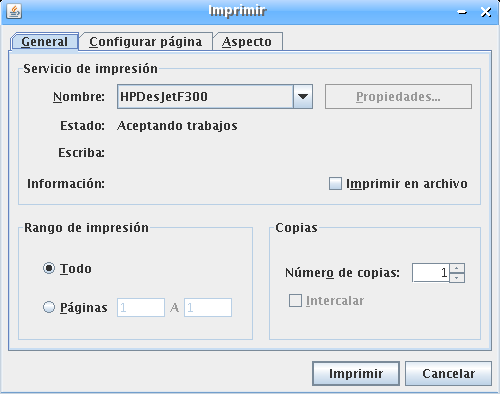
\includegraphics[scale=0.3]{Imagenes/02_Caracteristicas/VentanaImpresion_01.png}
      \end{center}
   \item \textbf{Configurar P\'agina}: Tipo de papel, Origen del papel,
      Orientaci\'on de la Hoja y M\'argenes
      \begin{center}
         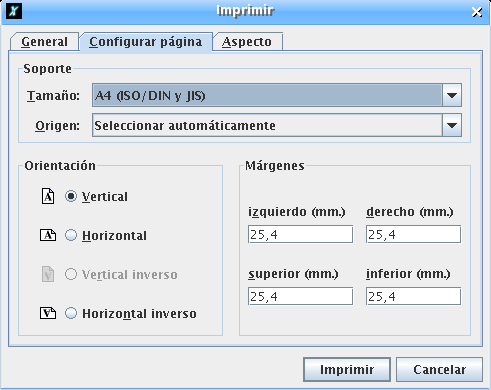
\includegraphics[scale=0.3]{Imagenes/02_Caracteristicas/VentanaImpresion_02.png}
      \end{center}
   \item \textbf{Aspecto}: Color (cuando disponible), Calidad, Caras y otros
      Atributos 
      \begin{center}
         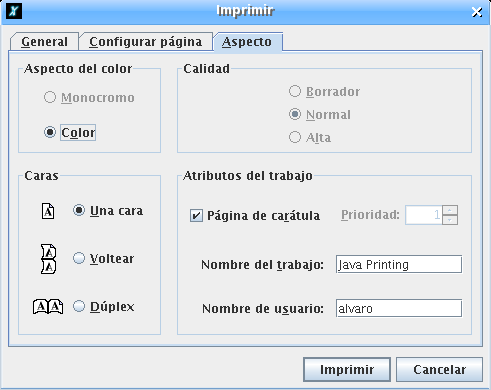
\includegraphics[scale=0.3]{Imagenes/02_Caracteristicas/VentanaImpresion_03.png}
      \end{center}
\end{itemize}

\section{Salir}
   \label{Salir}
   \index{Salir}

Para salir simplemente seleccionamos: \textbf{Archivo} $\rightarrow$ \textbf{Salir},
o hacemos \textit{click} en en el icono de cierre 
(
\includegraphics[scale=0.4]{Imagenes/02_Caracteristicas/cerrar.png}). \textsc{XLogo} presentar\'a
una ventana de confirmaci\'on: 
\begin{center}
   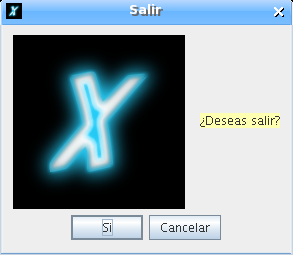
\includegraphics[scale=0.4]{Imagenes/02_Caracteristicas/SalirXLogo.png}
\end{center}
Pulsamos \texttt{S\'i} y termina la ejecuci\'on.
